
\documentclass[journal]{IEEEtran}

\usepackage{epsfig,graphicx,lineno,amssymb,mdwmath,array,amsmath}
% \usepackage{subfigure}
\usepackage{multirow}
\usepackage{xcolor}
\usepackage{cite}
\usepackage{epstopdf}
\usepackage{latexsym, bm}
\usepackage{algorithm}
\usepackage{algorithmicx}
\usepackage{algpseudocode}
\usepackage[utf8]{inputenc}
\usepackage[T1]{fontenc}
\usepackage{listings}

\usepackage[font=footnotesize]{subfig}
\usepackage{stfloats}


\definecolor{pblue}{rgb}{0.13,0.13,1}
\definecolor{pgreen}{rgb}{0,0.5,0}
\definecolor{pred}{rgb}{0.9,0,0}
\definecolor{pgrey}{rgb}{0.46,0.45,0.48}
\lstset{
  language=Java,
  frame=single,
  emph={enableRssiPolling},
%   emphstyle=\textbf,
  emphstyle=\color{red},
  showspaces=false,
  showtabs=false,
  breaklines=true,
  showstringspaces=false,
  breakatwhitespace=true,
  commentstyle=\color{pgreen},
  keywordstyle=\color{pblue},
  stringstyle=\color{pred},
%   basicstyle=\ttfamily,
  basicstyle=\small,
  stringstyle=\ttfamily,
  moredelim=[il][\textcolor{pgrey}]{$1$},
  moredelim=[is][\textcolor{pgrey}]{\%\%}{\%\%},
  numbers=left, numberstyle=\tiny, stepnumber=1, numbersep=5pt
}


\newtheorem{mydef}{Definition}
\newtheorem{mylem}{Lemma}
\newtheorem{mythm}{Theorem}
\newtheorem{cor}{Corollary}

\hyphenation{op-tical net-works semi-conduc-tor}

\makeatletter       %for algorithm
\def\BState{\State\hskip-\ALG@thistlm} %for algorithm
\makeatother %for algorithm

\algnewcommand\algorithmicswitch{\textbf{switch}}
\algnewcommand\algorithmiccase{\textbf{case}}

\algblockdefx[Name1]{SWITCH}{ENDSWITCH}%
%   [1]{\textbf{switch} #1 \textbf{do}}%
 [1]{\textbf{switch} #1}%
  {\textbf{end switch}}
\algblockdefx[Name2]{CASE}{ENDCASE}%
  [1]{\textbf{case} #1 \textbf{do}}%
  {\textbf{end case}}

\begin{document}
%
% paper title
% can use linebreaks \\ within to get better formatting as desired
% Do not put math or special symbols in the title.
\title{Green Wi-Fi: Rethinking About Energy Savings On Smartphones From A Usage Perspective}
%
\author{Lunde~Chen,
        ~Huan~Li*,~\IEEEmembership{Member,~IEEE}% <-this % stops a space
\thanks{*Corresponding Author: Dr. H. Li (email: lihuan@buaa.edu.cn),  is with the School
of Computer Science and Engineering, Beihang University, Beijing,
China 100191.
% ,  e-mail: lihuan@buaa.edu.cn
}% <-this % stops a space
\thanks{L. Chen is with with the School of Computer Science and Engineering and Ecole Centrale de P\'{e}kin, Beihang University, Beijing, China 100191.}
% <-this % stops a space
%\thanks{Manuscript received October 7, 2014.}
}

% The paper headers
\markboth{MobiSys'}%%Journal of \LaTeX\ Class Files,~Vol.~11, No.~4, December~2012}%
{Shell \MakeLowercase{\textit{et al.}}: Bare Demo of IEEEtran.cls for Journals}
\maketitle

\begin{abstract}

\end{abstract}

% Note that keywords are not normally used for peerreview papers.
\begin{IEEEkeywords}
Rssi, Energy saving, Wi-Fi, 
\end{IEEEkeywords}

\IEEEpeerreviewmaketitle

\section{Introduction}
%\IEEEPARstart{S}{martphones} are becoming increasingly popular and have emerged as a particularly appealing platform for network
% applications, especially through Wi-Fi interface.
%However, these light-weighted and easy-to-carry mobile devices are constrained by their limited battery capacity.
\section{Wi-Fi Energy Consumption  From A Usage Perspective}
While the energy consumption of Wi-Fi can be modelled with packet-level information and other factors, 
we find that the dominating factor of Wi-Fi energy consumption comes from the bursts of traffic.
For example, in our previous work of achieving energy saving of Wi-Fi regarding to Rssi, we found that 
Wi-Fi energy consumption can be seen as proportional to the time it takes to download a file. 

As a result, to achieve energy saving, the key is that the bursts of data should be smart.
We investigate the key factors that influence the burstness of Wi-Fi. 
We determine that Rssi, data scheduling and smartphone usage play important roles.
\subsection{Rssi}

\begin{figure}
\centering
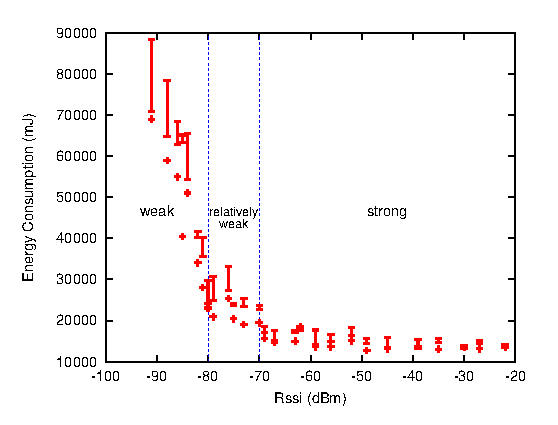
\includegraphics[scale=0.95]{rssi_energy.eps}
\caption{Energy Consumption in different Rssi}
\label{rssi_energy}
\end{figure}

\begin{figure}
\centering
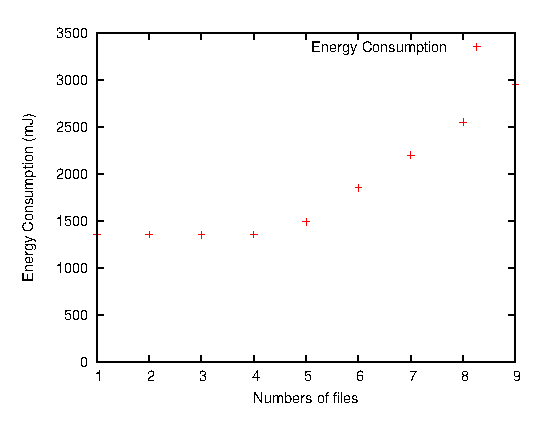
\includegraphics[scale=0.95]{energy_number_of_downloads_orderof_400KB.eps}
\caption{Energy Consumption of Batching Downloading Several File}
\label{energy_number_of_downloads_orderof_400KB}
\end{figure}

\subsection{Data Scheduling}
For delay-tolerant data, batching them in a single burst can achieve significant energy saving. 
As we measured, downloading a file of 500 KB via HTTP cost the same energy as downloading 
4 files of 500 KB, as shown in Fig. \ref{energy_number_of_downloads_orderof_400KB}. On the one hand, Wi-Fi has very high throughput, and mobile data is generally of 
small size [3]. On the other hand, 97\% of mobile data is HTTP-based [3], 
which involves the initiation and the closure of HTTP connection, batching several 
HTTP data can make the time of download overlap. The overhead of maintaining multiple TCP connections
can be ignored.
\subsection{Smartphone Usage}
As we found, when the smartphone is in usage, the energy cost of Wi-Fi interface is lower than when the phone 
is screen-locked. So we can exploit this for energy saving.

Applications with network permission could open the Wi-Fi interface periodically for little data transmission, even when the phone is screen-locked and not used. This could represent a huge amount of energy consumption, especially when many such applications are installed in the smartphone.
However, as [1] shows, Android smartphone users usually use only 20\% of their installed applications the most frequently, but rarely use other applications.
So we could use Iptables to block the Internet access of these rarely-used applications to save energy.

\begin{figure}
\centering
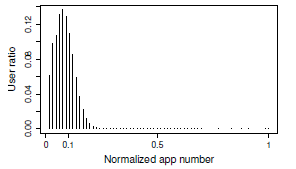
\includegraphics[scale=0.95]{application_utilisation_android.png}
\caption{User distribution of app diversity of Android phones [1]}
\label{application_utilisation_android}
\end{figure}

\section{Green Wi-Fi Design}

\subsection{Architecture}
\begin{figure}
\centering
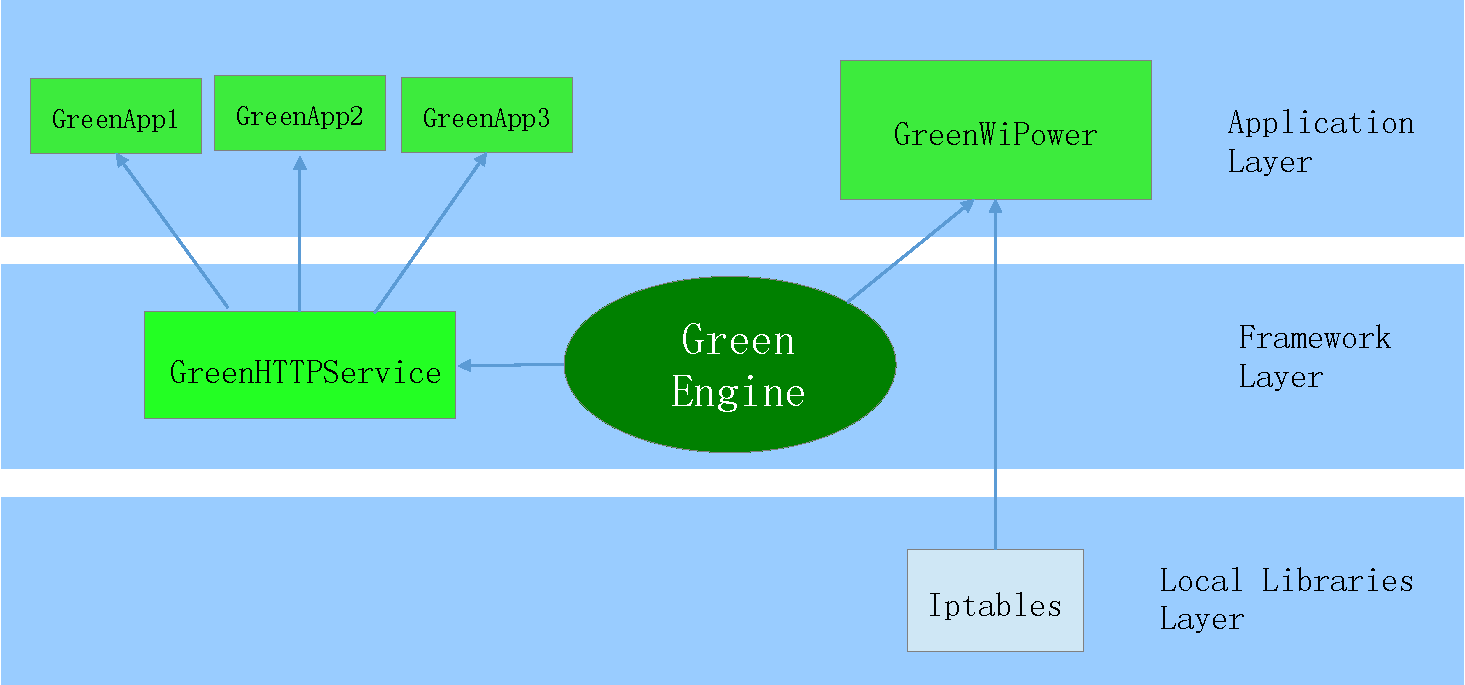
\includegraphics[scale=0.35]{architecture.pdf}
\caption{Architecture of Green Wi-Fi}
\label{architecture}
\end{figure}

As shown in Fig. \ref{architecture}.
\subsection{Decision Engine}
The input of the decision engine: Rssi, Wi-Fi SSID, HTTP data size and their delay-tolerance, application usage history data, 
remained battery.

The intermediate output of the decision engine: FSM of Wi-Fi state, max throughput of Wi-Fi AP

The final output of the decision engine: Transfer data or not, which applications to block/unblock with Iptables.
% 较少使用的,并且有 Network 权限的 app, 则用 iptables 给 block 掉。
%
%
\subsection{Implementation}
Implementation: The Green Engine, the GreenHTTPService framework, multiple test applications GreenApp1, GreenApp2, GreenApp3 ... and also GreenWiPower which blocks the Internet access of rarely-used applications installed by a specific user.

\section{Experimental Results}
Comparision of battery lifetime with and without Green Wi-Fi.

\section{Related Work}
\section{Conclusions} 
\section*{Acknowledgement}

This work is supported by the National Nature Science Foundation of China, NSFC (Grant No. 61170293) 
and the International Science \& Technology Cooperation Program of China, 
Ministry of Science and Technology of China (Grant No. 2014DFG12370).

\ifCLASSOPTIONcaptionsoff
  \newpage
\fi
\begin{thebibliography}{1}
\bibitem{biblio1}
Yinzhou Li, Jie Yang, Nirwan Ansari \emph{Cellular Smartphone Traffic and User Behavior Analysis}, 
\hskip 1em plus
  0.5em minus 0.4em\relax IEEE ICC 2014 - Communication QoS, Reliability and Modeling Symposium

\bibitem{biblio2}
Yu Xiao, Yong Cui, Petri Savolainen, et al. \emph{Modeling Energy Consumption of Data Transmission over Wi-Fi}, 
\hskip 1em plus
  0.5em minus 0.4em\relax IEEE TRANSACTIONS ON MOBILE COMPUTING
  
\bibitem{biblio3}
Hossein Falaki, Dimitrios Lymberopoulos, Ratul Mahajan  \emph{A First Look at Traffic on Smartphones}, 
\hskip 1em plus
  0.5em minus 0.4em\relax IMC’10,

\end{thebibliography}
\end{document}


